% lint-skip: 未完成ステータス（figure/table caption 未対応，人手チェック時に解消予定）
\documentclass[../../main.tex]{subfiles}
\begin{document}

\begin{flushright}
  \footnotesize\textit{【自動文字起こし・要確認】}
\end{flushright}

\noindent
[\textbf{解}] 右図のような座標平面を考える．

\begin{figure}[htb]
  \centering
  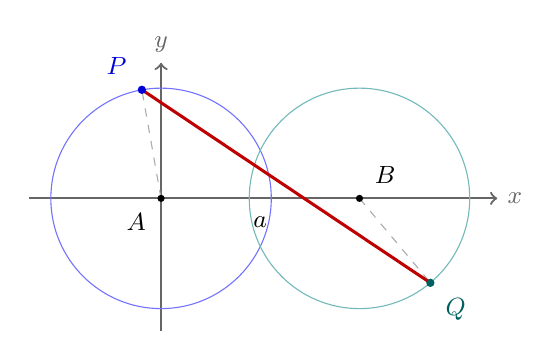
\begin{tikzpicture}[x=1.4cm, y=1.4cm,
    every node/.style={font=\small}]
    % Illustrative positions for a=1.8 and theta=50 degrees.
    \coordinate (A) at (0,0);
    \coordinate (B) at (1.8,0);
    \coordinate (P) at (-0.174,0.985);
    \coordinate (Q) at (2.443,-0.766);
    \draw[->, thick, gray!80!black] (-1.2,0)--(3.05,0)
    node[right] {$x$};
    \draw[->, thick, gray!80!black] (0,-1.2)--(0,1.23)
    node[above] {$y$};
    \draw[thin, blue!55] (A) circle[radius=1];
    \draw[thin, teal!55] (B) circle[radius=1];
    \draw[dashed, gray!65] (A)--(P) (B)--(Q);
    \draw[line width=1.1pt, red!75!black] (P)--(Q);
    \fill (A) circle(1.3pt) node[below left=2pt] {$A$};
    \fill (B) circle(1.3pt) node[above right=2pt] {$B$};
    \fill[blue!85!black] (P) circle(1.5pt)
    node[above left=2pt] {$P$};
    \fill[teal!75!black] (Q) circle(1.5pt)
    node[below right=2pt] {$Q$};
    \node[below=3pt] at (0.9,0) {$a$};
  \end{tikzpicture}
  \caption{座標の取り方と二つの単位円上の点 $P,Q$}
  \label{fig:1966_4_positions}
\end{figure}

\noindent
すると $0 \le \theta < 2\pi$ として
\[
  \vec{AP} =
  \begin{pmatrix} \cos 2\theta \\ \sin 2\theta
  \end{pmatrix}, \quad
  \vec{AQ} =
  \begin{pmatrix} a \\ 0
  \end{pmatrix} +
  \begin{pmatrix} \cos(-\theta) \\ \sin(-\theta)
  \end{pmatrix}
\]
とおけるから
\[
  \vec{PQ} =
  \begin{pmatrix} a + \cos\theta - \cos 2\theta \\ -\sin\theta - \sin 2\theta
  \end{pmatrix}
\]
$|\vec{PQ}| \ge 0$ から，$|\vec{PQ}|^2$ が最大の時，$|\vec{PQ}|$ も最大．以下 $\cos\theta = c, \sin\theta = s$ と略記して，
\begin{align}
  |\vec{PQ}|^2 &= \{ a + c - (2c^2 - 1) \}^2 + (-s - 2cs)^2 \\
  &= (-2c^2 + c + a + 1)^2 + s^2(1 + 2c)^2 \\
  &= 4c^4 - 4c^3 - (4a + 3)c^2 + 2(a + 1)c + (a + 1)^2 + (1 - c^2)(4c^2 + 4c + 1) \\
  &= -4ac^2 + 2(a - 1)c + (a^2 + 2a + 2) \equiv f(c)
\end{align}
以下 $f(c)$ の最大値を求める．$a > 0$ に注意して，軸の大きさで場合分けする．

\begin{figure}[htb]
  \centering
  \begin{tikzpicture}[x=3cm, y=1.6cm,
    every node/.style={font=\small}]
    % The axis of f(c), viewed as a function of a>0.
    \draw[->, thick, gray!80!black] (-0.08,0)--(2.45,0)
    node[right] {$a$};
    \draw[->, thick, gray!80!black] (0,-1.65)--(0,0.48)
    node[above] {$c$};
    \draw[dashed, gray!60] (0,0.25)--(2.3,0.25);
    \draw[dashed, gray!60] (0,-1)--(2.3,-1);
    \draw[line width=1.3pt, blue!85!black,
    domain=0.14:2.3, samples=120, smooth]
    plot (\x,{0.25-0.25/\x});
    \draw[dashed, gray!65] (0.2,0)--(0.2,-1);
    \fill[red!80!black] (0.2,-1) circle(1.5pt);
    \fill[teal!75!black] (1,0) circle(1.5pt);
    \node[left=2pt, font=\footnotesize] at (0,-1) {$-1$};
    \node[left=2pt, font=\footnotesize] at (0,0.25) {$\frac14$};
    \node[above left=2pt, font=\footnotesize] at (0.2,0)
    {$\frac15$};
    \node[below=2pt, font=\footnotesize] at (1,0) {$1$};
    \node[blue!85!black, font=\footnotesize] at (1.55,-0.24)
    {$c=\dfrac{a-1}{4a}$};
  \end{tikzpicture}
  \caption{$f(c)$ の軸と $-1\le c\le1$ の位置関係}
  \label{fig:1966_4_axis_position}
\end{figure}

\begin{enumerate}
  \item[$1^\circ$] $0 < a \le \dfrac{1}{5}$ の時
    \[
      \max f(c) = f(-1) = (a - 2)^2
    \]
  \item[$2^\circ$] $\dfrac{1}{5} \le a$ の時
    \[
      \max f(c) = f\left(\dfrac{a-1}{4a}\right) = a^2 + \dfrac{9}{4}a + \dfrac{3}{2} + \dfrac{1}{4a}
    \]
\end{enumerate}
以上から，
\[
  \begin{cases}
    0 < a \le \dfrac{1}{5} \text{の時} & 2 - a \\
    \dfrac{1}{5} \le a \text{の時} & \sqrt{a^2 + \dfrac{9}{4}a + \dfrac{3}{2} + \dfrac{1}{4a}}
  \end{cases}
\]

\newpage

\end{document}
